\documentclass[11pt]{scrartcl}

\usepackage[utf8]{inputenc}
\usepackage{csquotes}
\usepackage[british]{babel}
\usepackage[dvipsnames]{xcolor}
\usepackage{a4wide}
\usepackage{xspace}
\usepackage{amsmath}
\usepackage{graphicx}
\usepackage{algorithm}
\usepackage{algpseudocode}
\usepackage{tikz}
\usetikzlibrary{shapes.misc, positioning}
\usepackage{listings}
\usepackage{verbatim}
\usepackage{listings}
\usepackage{hyperref}
\usepackage{markdown}
\usepackage{placeins}

\usepackage[backend=biber]{biblatex}
\addbibresource{report.bib}

\graphicspath{ {./images} }

\markdownSetup{pipeTables,tableCaptions}
\definecolor{dkgreen}{rgb}{0,0.6,0}
\definecolor{gray}{rgb}{0.5,0.5,0.5}
\definecolor{mauve}{rgb}{0.58,0,0.82}


\lstset{frame=tb,
  language=Java,
  aboveskip=3mm,
  belowskip=3mm,
  showstringspaces=false,
  columns=flexible,
  basicstyle={\small\ttfamily},
  numbers=left,
  numberstyle=\tiny\color{gray},
  keywordstyle=\color{blue},
  commentstyle=\color{green},
  stringstyle=\color{mauve},
  breaklines=true,
  breakatwhitespace=true,
  tabsize=3
}
\hypersetup{
    colorlinks=true,
    frenchlinks=false,
    bookmarksopen=true,
    breaklinks=true,
    linkcolor=black,
    urlcolor=black,
    citecolor=black,
    pdftitle=Project proposal,
    pdfauthor={Tobias Eilertsen}
}

\lstdefinelanguage{kotlin}{
  comment=[l]{//},
  commentstyle={\color{gray}\ttfamily},
  emph={delegate, filter, first, firstOrNull, forEach, lazy, map, mapNotNull, println, return@},
  emphstyle={\color{OrangeRed}},
  identifierstyle=\color{black},
  keywords={abstract, actual, as, as?, break, by, class, companion, continue, data, do, dynamic, else, enum, expect, false, final, for, fun, get, if, import, in, interface, internal, is, null, object, override, package, private, public, return, set, super, suspend, this, throw, true, try, typealias, val, var, vararg, when, where, while,lateinit},
  keywordstyle={\color{blue}\bfseries},
  morecomment=[s]{/*}{*/},
  morestring=[b]",
  morestring=[s]{"""*}{*"""},
  morekeywords={[2]{@Autowired, @RestController, @RequestMapping, @Bean, Array, Byte, Double, Float, Int, Integer, Iterable, Long, Runnable, Short, String, @Valid, @RequestBody,@PostMapping, @GetMapping, @DeleteMapping, @PutMapping}},
  keywordstyle={[2]\color{BurntOrange}\bfseries},
  morekeywords={[3]{accountService, account, window,id,accountRequest}},
  keywordstyle={[3]{\color{DarkOrchid}\bfseries}},
  morekeywords={[4]{AccountRequest, AccountResponse, AccountController,AccountService,AccountCreationRequest}},
  keywordstyle={[4]{\color{Periwinkle}\textbf}},
  sensitive=true,
  stringstyle={\color{ForestGreen}\ttfamily},
}
\begin{document}

\title{Project proposal}
\subtitle{Preoperative fracture surgery using virtual reality}

\author{Tobias Eilertsen}
\maketitle


\section*{Supervisors}
\begin{itemize}
  \item Harald Soleim
  \item Atle Geitung
  \item Daniel Patel
\end{itemize}
\section*{Collaborator}
\begin{itemize}
  \item Haukeland Universitetssykehus, medisinsk teknisk avdeling
\end{itemize}

\begin{abstract}
Before and during a surgery, it is important for medical personnel to have a
good understanding of the anatomy of a patient. A better understanding can
lead to a less invasive surgery with less risk of implications.
The goal of this project is to create a better way for medical personnel to
inspect 3d models, making surgeries easier and safer.
\end{abstract}

\newpage
\section{introduction}


\subsection{introduction}

When a hospital receives a injured patient that needs orthopedic surgery, a CT scan is
often performed. The CT images are then displayed as a set of images or a 3D model on a computer. This helps
the medical personnel plan the surgery by inspecting bone mass.
If a surgeon has a good understanding of the anatomy related to the fracture,
it is possible to perform a surgery that has less risk of complications or requires less resources.


A problem with visualising the model in 2D the limited understanding of what
the bone actually looks like, because of the lack of scale and depth. A
possible solution is visualising the model in Augumented Reality or Virtual
Reality to give medical personnel a good feel for what the problem area actually looks like.

\subsection{Research Questions}
VR has many potential benefits, and it is possible that the surgery planning
process can use some of these. As the users are already looking at 3d models in
2d screens, visualising in VR could improve the surgeons overview and improve the patients safety. The entire planning process could also be more effective, by removing or reducing the need for 3D printed models, especially in cases with limited time. Therefore the possible research questions are as follows:

How Can VR technology improve surgery planning by making the process safer or more effective?
How Can VR technology give some of the same benefits as 3D printing gives today at a lower cost?


\subsection{Expected Results}
The project should include a VR prototype of a standard where it is
user friendly enough to test with non technical subjects and with functionality
that is comparable to the usecases of a printed model.
The prototype will be tested on medical personnel to investigate the impact on the users anatomical understanding, how it effects the surgery and the efficiency of the planning process. 
The application should be available for further development and/or study.

The resulting report will include interviews and a conclusion describing what the
performance of the VR viewer is compared to existing solutions, and whether VR is a
valuable tool for surgery planning.  

\subsection{Related works}

There currently exists several alternatives to viewing medical data in VR, here are some of the alternatives:

Medical Holodeck~\cite{medical_holodeck_medicalholodeck_nodate} is made for surgeons to plan surgeries and education.

An Augumented reality viewer called Dicom Director also exists, but is not yet approved for clinical use.\cite{dicomdirectorcom_surgeons_nodate}

Other similar solutions are Materialise\cite{materialise_medical_nodate} and
Ceevra\cite{ceevra_inc_using_2019}.

Most current solutions are closed source premium services targeted at enterprise/medical institutions. Many of them are not yet approved for clinical use, and current solutions are difficult to use for people not used to Virtual Reality \emph{cite needed}


Some free general purpose VR viewers for 3D models also exist, but I have not found any with features related to medical use, collaboration or plannning.

A study in visualising Patient data with VR \cite{vertemati_virtual_2019} implemented a VR viewer for DICOM data and tried to measure anatomical uderstanding compared to 2D images. The study did not investigate the efficiency of the planning phase (loading the model into the software took 1 hour), and it did not do a comparison to 3D printing.

\section{ background }

\subsection{ existing solutions}


\subsubsection { 3D printing }

An alternative to digital representation is to print the 3d model to inspect it physically \cite{mishra_virtual_2019}. This has many advantages, such as the surgeon being able to physically hold the bodypart, measure the model, try out equipment and practice with it.
The biggest drawback to 3D printing is that the printing process can take more than 24 hours depending on the model, which in some cases is too long. Another drawback is not having any digital tools such as transparency, displaying cross sections or being able to alter the model in any way. Having a physical model in plastic also means it needs support structures, which can get in the way or create a inaccurate representation of the fracture.

A possible future usecase for this project is taking a quick look at a model in VR, and then deciding if a printed model is necessary, potentially saving time and resources.

\subsubsection{2D viewer}

There exists a wide range of computer programs to inspect CT images as 3D models, using the computer to interact with the model.
The current solution used by Helse Vest is materialise \cite{materialise}. Using a 2D viewer is fast and simple, but lacks the depth and scale of VR.


\section{Literature and References}

\begin{itemize}
\item Mini invasiv behandling av brudd i hælbeinet ved hjelp av 3D printing:
\begin{description}
\item Norwegian presentation showing how 3d Printing is used to improve surgery planning
\end{description}


\item Virtual preoperative planning and 3D printing are valuable for the management of complex orthopaedic trauma
\begin{description}
\item Article describing how 3D printing in planning can reduce surgical morbidity
\end{description}


\item A Virtual Reality Environment to Visualize Three-Dimensional Patient-Specific Models by a Mobile Head-Mounted Display
\begin{description}
\item Article testing the usability of viewing models in VR for surgeons and
    interviewing participants.
\end{description}


\item A collaborative virtual reality environment for liver surgery planning
\begin{description}
\item Article using VR specifically for liver surgery planning.
\end{description}

\item Using Virtual Reality (VR) Models for Preoperative Planning
\begin{description}
\item Quantitative study with randomized participants from surgical field
    measuring the impact of VR in pre op phase based on surgery duration.
\end{description}
\end{itemize}



\section{Research Method}
Firstly, a prototype Vr viewer will be created with the help of related
open-source frameworks/software and guidance from both orthopedic surgeons and
developers with experience from medical technology.

To answer the research question, it is necessary to measure the
performance of the final application. This thesis will use qualitative methods
by interviewing related personnel to investigate the performance including
anatomical understanding, cooperation, and the effectiveness of the planning
process.
This will also be put in context to the existing solutions, possibly
by doing a direct comparsion by using a 3D model, printed model and VR viewer
on the same case.

\section{Thesis Outline}
\begin{itemize}

\item Introduction (7-9 pages)

\begin{description}
\item short description of how vr can be used to plan surgery
\end{description}

\item Background(10-12 pages)

\begin{description}
\item Description of related medical processes, surgery and surgery planning.
\item describe current state of 3D printing and Vr usage in medical field.
\end{description}

\item problem(2-3 pages)

\begin{description}
\item Describe what the application hopes to solve
\end{description}

\item method(3-4 pages)

\begin{description}
\item How the application is created and how final result will be measured
\end{description}

\item Implementation(10-15 pages)

\begin{description}
\item how the final application is designed
\end{description}

\item Evaluation (10-12 pages)

\begin{description}
\item results after final evaluation
\end{description}

\item Conclusion and Future Work(5 pages)

\begin{description}
\item if project was a success and how VR in pre op planning can be improved
\end{description}

\end{itemize}

\section{Project Plan}

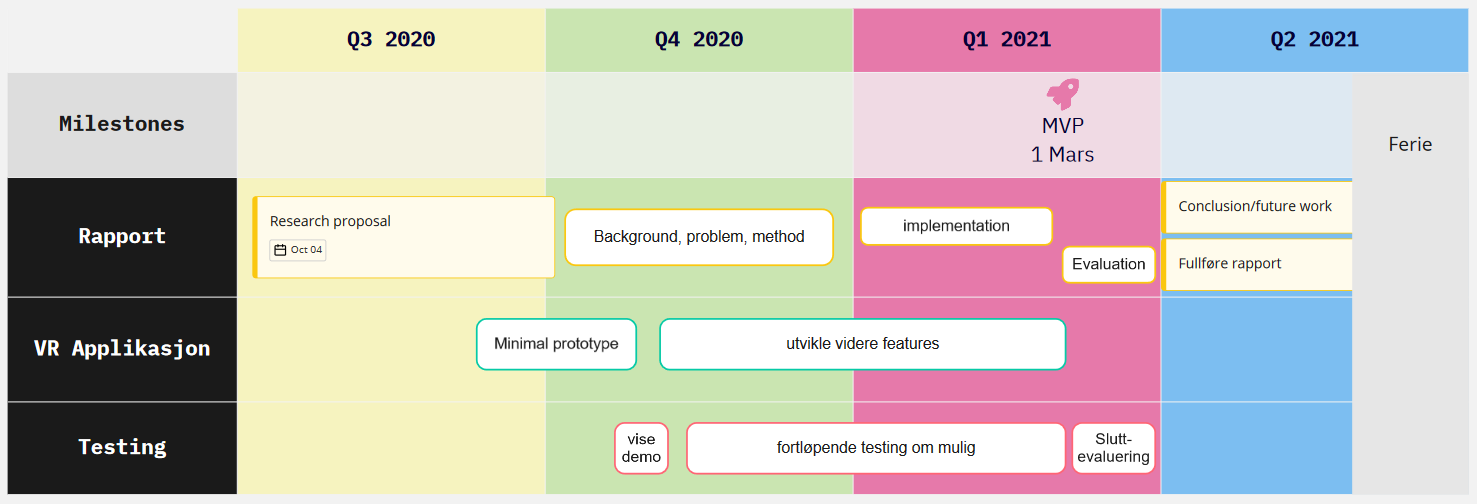
\includegraphics[width=\textwidth]{timeline.png}

\section{Conclusions and Outlook}

This report will hopefully answer some questions regarding the usability of Virtual Reality in
surgeries, and bring more awareness and interest towards potential future uses
of Virtual Reality. 

To get an valid and interesting result it is necessary that the application is of a
decent quality. The resulting application should be available for further
development and study.


\section{Literature and References}


\printbibliography

\end{document}
